\documentclass[11pt]{standalone}
\usepackage{tikz}
\usepackage{amssymb}
\begin{document}
% GEOMIRA export: TikZ. One unit is 46.666667bp (62.222222 px on screen).
% Needs \usepackage{tikz} and \usepackage{amssymb}.
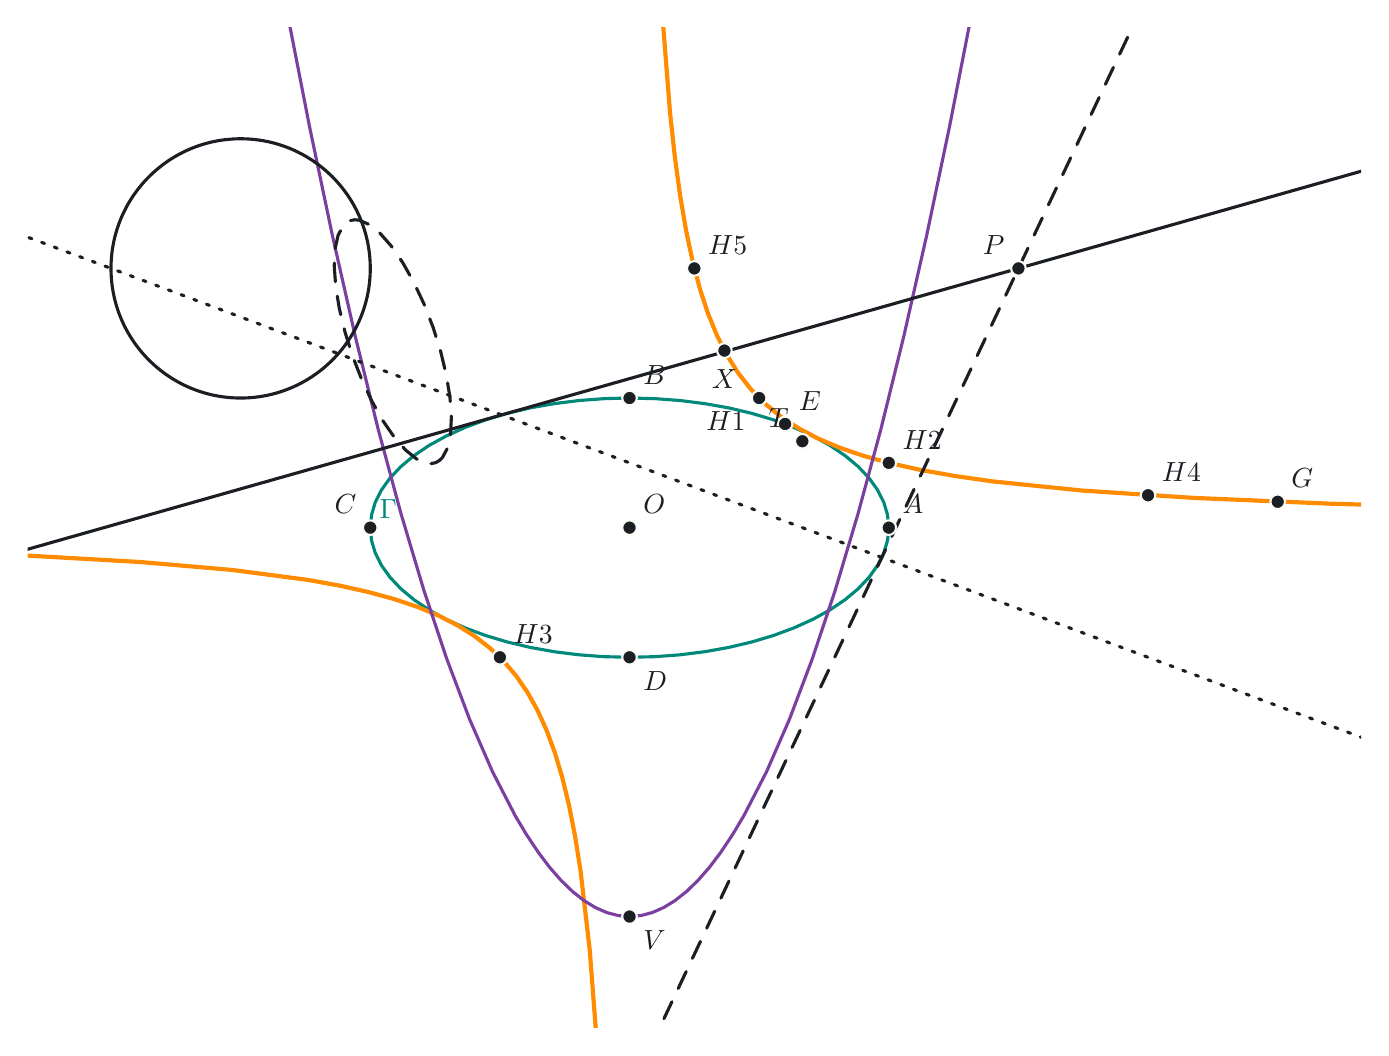
\begin{tikzpicture}[x=46.666667bp, y=46.666667bp, line cap=round, line join=round]
\definecolor{gmc0}{HTML}{00897B}
\definecolor{gmc1}{HTML}{FF8C00}
\definecolor{gmc2}{HTML}{7B3FA0}
\definecolor{gmc3}{HTML}{1B1F24}
\definecolor{gmc4}{HTML}{FBFBF8}
\clip (-4.6429,-3.8571) rectangle (5.6429,3.8571);
% e
\draw[gmc0, line width=1.125bp] (2,0) -- (1.9904,0.098) -- (1.9616,0.1951) -- (1.9139,0.2903) -- (1.8478,0.3827) -- (1.7638,0.4714) -- (1.6629,0.5556) -- (1.546,0.6344) -- (1.4142,0.7071) -- (1.2688,0.773) -- (1.1111,0.8315) -- (0.9428,0.8819) -- (0.7654,0.9239) -- (0.5806,0.9569) -- (0.3902,0.9808) -- (0.196,0.9952) -- (0,1) -- (-0.196,0.9952) -- (-0.3902,0.9808) -- (-0.5806,0.9569) -- (-0.7654,0.9239) -- (-0.9428,0.8819) -- (-1.1111,0.8315) -- (-1.2688,0.773) -- (-1.4142,0.7071) -- (-1.546,0.6344) -- (-1.6629,0.5556) -- (-1.7638,0.4714) -- (-1.8478,0.3827) -- (-1.9139,0.2903) -- (-1.9616,0.1951) -- (-1.9904,0.098) -- (-2,0) -- (-1.9904,-0.098) -- (-1.9616,-0.1951) -- (-1.9139,-0.2903) -- (-1.8478,-0.3827) -- (-1.7638,-0.4714) -- (-1.6629,-0.5556) -- (-1.546,-0.6344) -- (-1.4142,-0.7071) -- (-1.2688,-0.773) -- (-1.1111,-0.8315) -- (-0.9428,-0.8819) -- (-0.7654,-0.9239) -- (-0.5806,-0.9569) -- (-0.3902,-0.9808) -- (-0.196,-0.9952) -- (0,-1) -- (0.196,-0.9952) -- (0.3902,-0.9808) -- (0.5806,-0.9569) -- (0.7654,-0.9239) -- (0.9428,-0.8819) -- (1.1111,-0.8315) -- (1.2688,-0.773) -- (1.4142,-0.7071) -- (1.546,-0.6344) -- (1.6629,-0.5556) -- (1.7638,-0.4714) -- (1.8478,-0.3827) -- (1.9139,-0.2903) -- (1.9616,-0.1951) -- (1.9904,-0.098) -- (2,0) -- cycle;
% h
\draw[gmc1, line width=1.5bp] (6.7357,0.1485) -- (5.41,0.1848) -- (4.3452,0.2301) -- (3.49,0.2865) -- (2.8031,0.3567) -- (2.5121,0.3981) -- (2.2514,0.4442) -- (2.0177,0.4956) -- (1.8083,0.553) -- (1.6206,0.6171) -- (1.4524,0.6885) -- (1.3016,0.7683) -- (1.1665,0.8573) -- (1.0454,0.9565) -- (0.9369,1.0673) -- (0.8397,1.1909) -- (0.7525,1.3289) -- (0.6744,1.4828) -- (0.6044,1.6545) -- (0.5417,1.8461) -- (0.4854,2.06) -- (0.4351,2.2985) -- (0.3899,2.5647) -- (0.3494,2.8618) -- (0.3132,3.1932) -- (0.2515,3.9757) -- (0.202,4.95);
\draw[gmc1, line width=1.5bp] (-0.202,-4.95) -- (-0.249,-4.0159) -- (-0.3069,-3.258) -- (-0.3783,-2.6432) -- (-0.42,-2.3808) -- (-0.4663,-2.1444) -- (-0.5177,-1.9315) -- (-0.5748,-1.7397) -- (-0.6382,-1.567) -- (-0.7085,-1.4114) -- (-0.7866,-1.2713) -- (-0.8733,-1.1451) -- (-0.9696,-1.0314) -- (-1.0764,-0.929) -- (-1.1951,-0.8368) -- (-1.3268,-0.7537) -- (-1.4731,-0.6788) -- (-1.6355,-0.6114) -- (-1.8157,-0.5507) -- (-2.0159,-0.4961) -- (-2.2381,-0.4468) -- (-2.4848,-0.4024) -- (-3.0628,-0.3265) -- (-3.7752,-0.2649) -- (-4.6533,-0.2149) -- (-5.7357,-0.1743);
% q
\draw[gmc2, line width=1.125bp] (2.8196,4.95) -- (2.6434,3.9873) -- (2.4671,3.0867) -- (2.2909,2.2482) -- (2.1147,1.4719) -- (1.9385,0.7576) -- (1.7622,0.1055) -- (1.586,-0.4846) -- (1.4098,-1.0125) -- (1.2336,-1.4783) -- (1.0573,-1.882) -- (0.8811,-2.2236) -- (0.793,-2.3711) -- (0.7049,-2.5031) -- (0.6168,-2.6196) -- (0.5287,-2.7205) -- (0.4406,-2.8059) -- (0.3524,-2.8758) -- (0.2643,-2.9301) -- (0.1762,-2.9689) -- (0.0881,-2.9922) -- (0,-3) -- (-0.0881,-2.9922) -- (-0.1762,-2.9689) -- (-0.2643,-2.9301) -- (-0.3524,-2.8758) -- (-0.4406,-2.8059) -- (-0.5287,-2.7205) -- (-0.6168,-2.6196) -- (-0.7049,-2.5031) -- (-0.793,-2.3711) -- (-0.8811,-2.2236) -- (-1.0573,-1.882) -- (-1.2336,-1.4783) -- (-1.4098,-1.0125) -- (-1.586,-0.4846) -- (-1.7622,0.1055) -- (-1.9385,0.7576) -- (-2.1147,1.4719) -- (-2.2909,2.2482) -- (-2.4671,3.0867) -- (-2.6434,3.9873) -- (-2.8196,4.95);
% w
\draw[gmc3, line width=1.125bp] (-2,2) arc[start angle=0, end angle=360, radius=1];
% w'
\draw[gmc3, line width=1.125bp, dash pattern=on 6.75bp off 5.25bp] (-1.4984,0.5006) -- (-1.4695,0.5157) -- (-1.444,0.5398) -- (-1.4043,0.6134) -- (-1.3808,0.7186) -- (-1.3744,0.8513) -- (-1.3854,1.0065) -- (-1.4133,1.1781) -- (-1.4571,1.3595) -- (-1.515,1.5439) -- (-1.5849,1.7241) -- (-1.6641,1.8931) -- (-1.7495,2.0445) -- (-1.8379,2.1725) -- (-1.9257,2.2722) -- (-2.0098,2.3397) -- (-2.0868,2.3723) -- (-2.1217,2.3752) -- (-2.1538,2.369) -- (-2.1827,2.3538) -- (-2.2082,2.3298) -- (-2.2479,2.2561) -- (-2.2714,2.1509) -- (-2.2778,2.0182) -- (-2.2668,1.8631) -- (-2.2389,1.6915) -- (-2.1951,1.51) -- (-2.1372,1.3257) -- (-2.0672,1.1455) -- (-1.9881,0.9765) -- (-1.9027,0.825) -- (-1.8143,0.697) -- (-1.7264,0.5974) -- (-1.6424,0.5299) -- (-1.5654,0.4972) -- (-1.5304,0.4944) -- (-1.4984,0.5006) -- cycle;
% t_1
\draw[gmc3, line width=1.125bp] (6.7357,3.059) -- (-5.7357,-0.4764);
% t_2
\draw[gmc3, line width=1.125bp, dash pattern=on 6.75bp off 5.25bp] (-0.2837,-4.95) -- (4.3938,4.95);
% p
\draw[gmc3, line width=1.125bp, dash pattern=on 1.125bp off 3.75bp] (6.7357,-2.0259) -- (-5.7357,2.6509);
% A
\filldraw[fill=gmc3, draw=gmc4, line width=0.75bp] (2,0) circle[radius=2.625bp];
% B
\filldraw[fill=gmc3, draw=gmc4, line width=0.75bp] (0,1) circle[radius=2.625bp];
% C
\filldraw[fill=gmc3, draw=gmc4, line width=0.75bp] (-2,0) circle[radius=2.625bp];
% D
\filldraw[fill=gmc3, draw=gmc4, line width=0.75bp] (0,-1) circle[radius=2.625bp];
% E
\filldraw[fill=gmc3, draw=gmc4, line width=0.75bp] (1.2,0.8) circle[radius=2.625bp];
% O
\filldraw[fill=gmc3, draw=gmc4, line width=0.75bp] (0,0) circle[radius=2.625bp];
% H1
\filldraw[fill=gmc3, draw=gmc4, line width=0.75bp] (1,1) circle[radius=2.625bp];
% H2
\filldraw[fill=gmc3, draw=gmc4, line width=0.75bp] (2,0.5) circle[radius=2.625bp];
% H3
\filldraw[fill=gmc3, draw=gmc4, line width=0.75bp] (-1,-1) circle[radius=2.625bp];
% H4
\filldraw[fill=gmc3, draw=gmc4, line width=0.75bp] (4,0.25) circle[radius=2.625bp];
% H5
\filldraw[fill=gmc3, draw=gmc4, line width=0.75bp] (0.5,2) circle[radius=2.625bp];
% G
\filldraw[fill=gmc3, draw=gmc4, line width=0.75bp] (5,0.2) circle[radius=2.625bp];
% P
\filldraw[fill=gmc3, draw=gmc4, line width=0.75bp] (3,2) circle[radius=2.625bp];
% T
\filldraw[fill=gmc3, draw=gmc4, line width=0.75bp] (1.3333,0.6667) circle[radius=2.625bp];
% X
\filldraw[fill=gmc3, draw=gmc4, line width=0.75bp] (0.7321,1.366) circle[radius=2.625bp];
% V
\filldraw[fill=gmc3, draw=gmc4, line width=0.75bp] (0,-3) circle[radius=2.625bp];
\node[anchor=south west, inner sep=0pt, text=gmc0] at (-1.9318,0.0682) {$\Gamma$}; % label of e
\node[anchor=south west, inner sep=0pt, text=gmc3] at (2.1023,0.1023) {$A$}; % label of A
\node[anchor=south west, inner sep=0pt, text=gmc3] at (0.1023,1.1023) {$B$}; % label of B
\node[anchor=south east, inner sep=0pt, text=gmc3] at (-2.1023,0.1023) {$C$}; % label of C
\node[anchor=north west, inner sep=0pt, text=gmc3] at (0.1023,-1.1023) {$D$}; % label of D
\node[anchor=south west, inner sep=0pt, text=gmc3] at (1.3023,0.9023) {$E$}; % label of E
\node[anchor=south west, inner sep=0pt, text=gmc3] at (0.1023,0.1023) {$O$}; % label of O
\node[anchor=north east, inner sep=0pt, text=gmc3] at (0.8977,0.8977) {$H1$}; % label of H1
\node[anchor=south west, inner sep=0pt, text=gmc3] at (2.1023,0.6023) {$H2$}; % label of H2
\node[anchor=south west, inner sep=0pt, text=gmc3] at (-0.8977,-0.8977) {$H3$}; % label of H3
\node[anchor=south west, inner sep=0pt, text=gmc3] at (4.1023,0.3523) {$H4$}; % label of H4
\node[anchor=south west, inner sep=0pt, text=gmc3] at (0.6023,2.1023) {$H5$}; % label of H5
\node[anchor=south west, inner sep=0pt, text=gmc3] at (5.1023,0.3023) {$G$}; % label of G
\node[anchor=south east, inner sep=0pt, text=gmc3] at (2.8977,2.1023) {$P$}; % label of P
\node[anchor=south east, inner sep=0pt, text=gmc3] at (1.2311,0.7689) {$T$}; % label of T
\node[anchor=north, inner sep=0pt, text=gmc3] at (0.7321,1.2214) {$X$}; % label of X
\node[anchor=north west, inner sep=0pt, text=gmc3] at (0.1023,-3.1023) {$V$}; % label of V
\end{tikzpicture}
\end{document}
